\documentclass[1p]{elsarticle_modified}
%\bibliographystyle{elsarticle-num}

%\usepackage[colorlinks]{hyperref}
%\usepackage{abbrmath_seonhwa} %\Abb, \Ascr, \Acal ,\Abf, \Afrak
\usepackage{amsfonts}
\usepackage{amssymb}
\usepackage{amsmath}
\usepackage{amsthm}
\usepackage{scalefnt}
\usepackage{amsbsy}
\usepackage{kotex}
\usepackage{caption}
\usepackage{subfig}
\usepackage{color}
\usepackage{graphicx}
\usepackage{xcolor} %% white, black, red, green, blue, cyan, magenta, yellow
\usepackage{float}
\usepackage{setspace}
\usepackage{hyperref}

\usepackage{tikz}
\usetikzlibrary{arrows}

\usepackage{multirow}
\usepackage{array} % fixed length table
\usepackage{hhline}

%%%%%%%%%%%%%%%%%%%%%
\makeatletter
\renewcommand*\env@matrix[1][\arraystretch]{%
	\edef\arraystretch{#1}%
	\hskip -\arraycolsep
	\let\@ifnextchar\new@ifnextchar
	\array{*\c@MaxMatrixCols c}}
\makeatother %https://tex.stackexchange.com/questions/14071/how-can-i-increase-the-line-spacing-in-a-matrix
%%%%%%%%%%%%%%%

\usepackage[normalem]{ulem}

\newcommand{\msout}[1]{\ifmmode\text{\sout{\ensuremath{#1}}}\else\sout{#1}\fi}
%SOURCE: \msout is \stkout macro in https://tex.stackexchange.com/questions/20609/strikeout-in-math-mode

\newcommand{\cancel}[1]{
	\ifmmode
	{\color{red}\msout{#1}}
	\else
	{\color{red}\sout{#1}}
	\fi
}

\newcommand{\add}[1]{
	{\color{blue}\uwave{#1}}
}

\newcommand{\replace}[2]{
	\ifmmode
	{\color{red}\msout{#1}}{\color{blue}\uwave{#2}}
	\else
	{\color{red}\sout{#1}}{\color{blue}\uwave{#2}}
	\fi
}

\newcommand{\Sol}{\mathcal{S}} %segment
\newcommand{\D}{D} %diagram
\newcommand{\A}{\mathcal{A}} %arc


%%%%%%%%%%%%%%%%%%%%%%%%%%%%%5 test

\def\sl{\operatorname{\textup{SL}}(2,\Cbb)}
\def\psl{\operatorname{\textup{PSL}}(2,\Cbb)}
\def\quan{\mkern 1mu \triangleright \mkern 1mu}

\theoremstyle{definition}
\newtheorem{thm}{Theorem}[section]
\newtheorem{prop}[thm]{Proposition}
\newtheorem{lem}[thm]{Lemma}
\newtheorem{ques}[thm]{Question}
\newtheorem{cor}[thm]{Corollary}
\newtheorem{defn}[thm]{Definition}
\newtheorem{exam}[thm]{Example}
\newtheorem{rmk}[thm]{Remark}
\newtheorem{alg}[thm]{Algorithm}

\newcommand{\I}{\sqrt{-1}}
\begin{document}

%\begin{frontmatter}
%
%\title{Boundary parabolic representations of knots up to 8 crossings}
%
%%% Group authors per affiliation:
%\author{Yunhi Cho} 
%\address{Department of Mathematics, University of Seoul, Seoul, Korea}
%\ead{yhcho@uos.ac.kr}
%
%
%\author{Seonhwa Kim} %\fnref{s_kim}}
%\address{Center for Geometry and Physics, Institute for Basic Science, Pohang, 37673, Korea}
%\ead{ryeona17@ibs.re.kr}
%
%\author{Hyuk Kim}
%\address{Department of Mathematical Sciences, Seoul National University, Seoul 08826, Korea}
%\ead{hyukkim@snu.ac.kr}
%
%\author{Seokbeom Yoon}
%\address{Department of Mathematical Sciences, Seoul National University, Seoul, 08826,  Korea}
%\ead{sbyoon15@snu.ac.kr}
%
%\begin{abstract}
%We find all boundary parabolic representation of knots up to 8 crossings.
%
%\end{abstract}
%\begin{keyword}
%    \MSC[2010] 57M25 
%\end{keyword}
%
%\end{frontmatter}

%\linenumbers
%\tableofcontents
%
\newcommand\colored[1]{\textcolor{white}{\rule[-0.35ex]{0.8em}{1.4ex}}\kern-0.8em\color{red} #1}%
%\newcommand\colored[1]{\textcolor{white}{ #1}\kern-2.17ex	\textcolor{white}{ #1}\kern-1.81ex	\textcolor{white}{ #1}\kern-2.15ex\color{red}#1	}

{\Large $\underline{12n_{0466}~(K12n_{0466})}$}

\setlength{\tabcolsep}{10pt}
\renewcommand{\arraystretch}{1.6}
\vspace{1cm}\begin{tabular}{m{100pt}>{\centering\arraybackslash}m{274pt}}
\multirow{5}{120pt}{
	\centering
	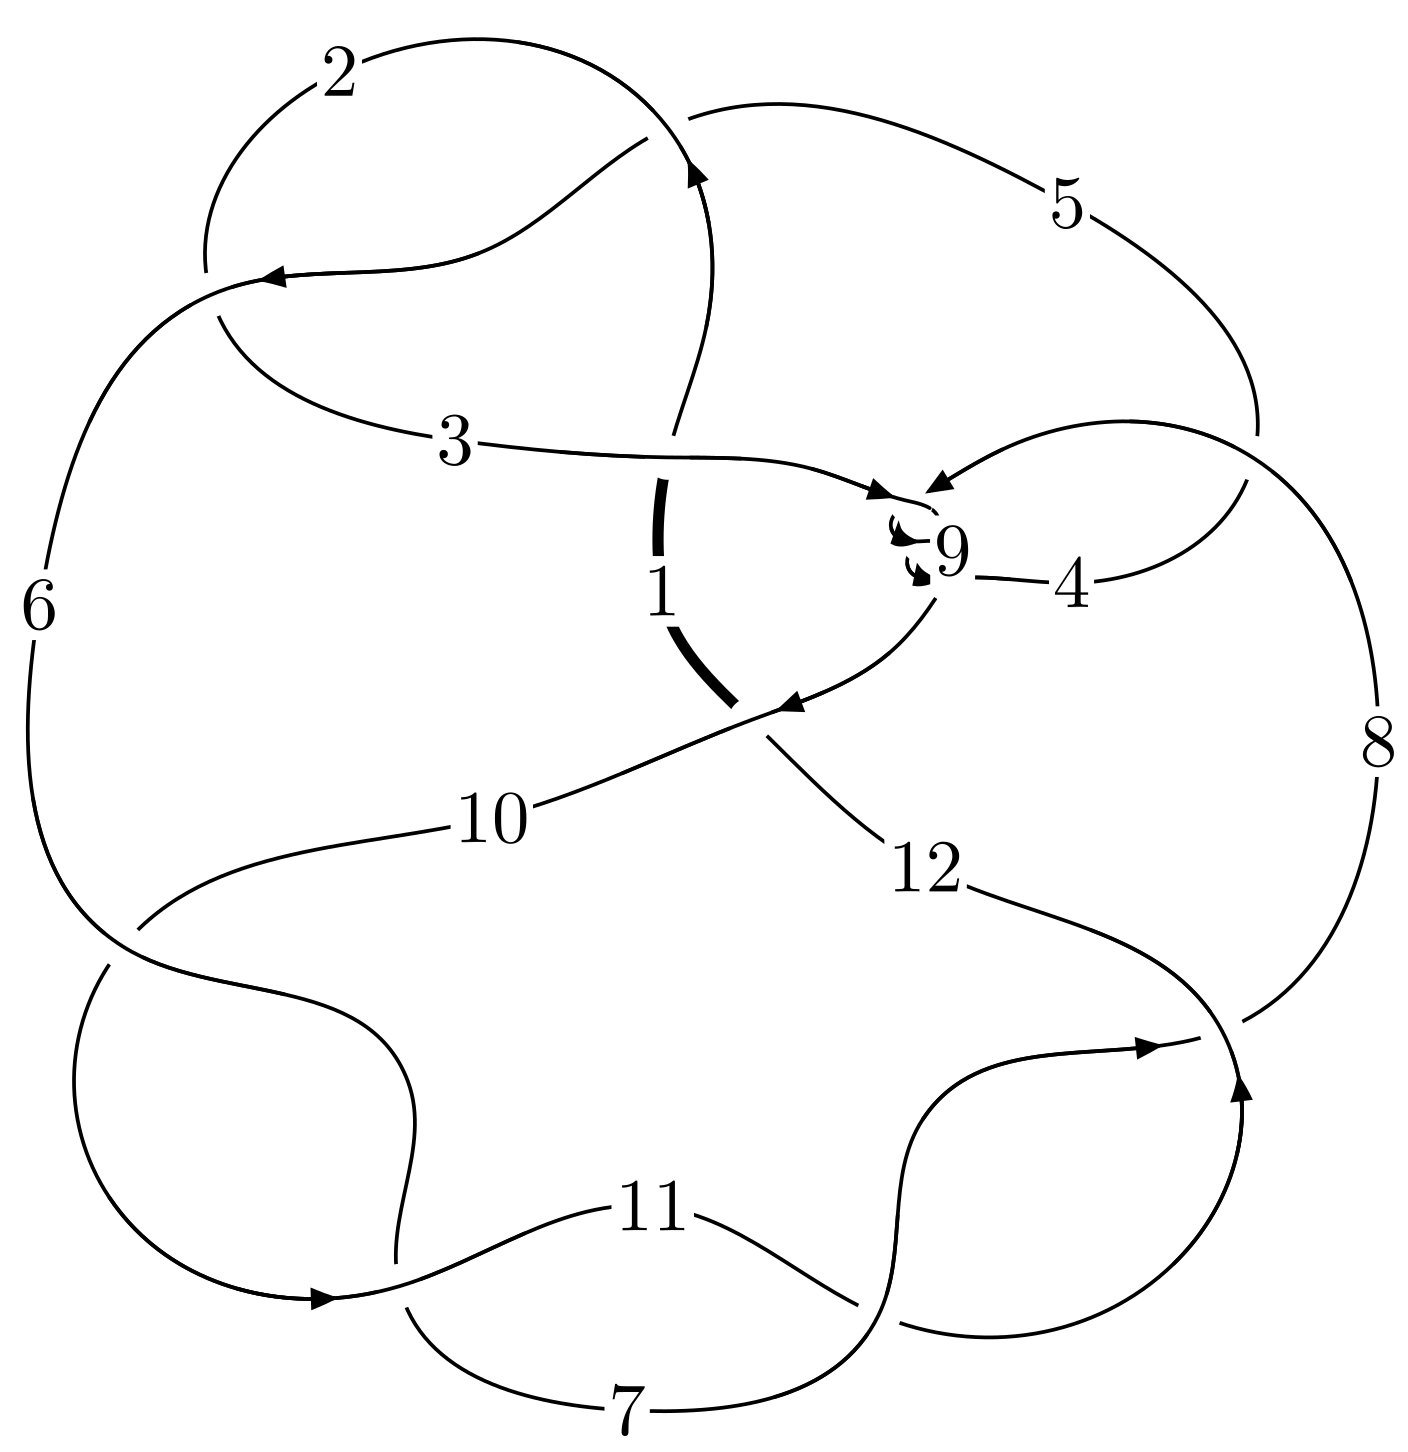
\includegraphics[width=112pt]{../../../GIT/diagram.site/Diagrams/png/2555_12n_0466.png}\\
\ \ \ A knot diagram\footnotemark}&
\allowdisplaybreaks
\textbf{Linearized knot diagam} \\
\cline{2-2}
 &
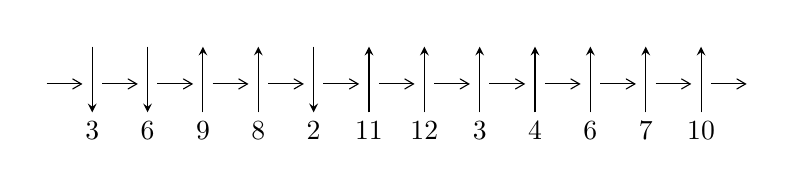
\begin{tikzpicture}[x=20pt, y=17pt]
	% nodes
	\node (C0) at (0, 0) {};
	\node (C1) at (1, 0) {};
	\node (C1U) at (1, +1) {};
	\node (C1D) at (1, -1) {3};

	\node (C2) at (2, 0) {};
	\node (C2U) at (2, +1) {};
	\node (C2D) at (2, -1) {6};

	\node (C3) at (3, 0) {};
	\node (C3U) at (3, +1) {};
	\node (C3D) at (3, -1) {9};

	\node (C4) at (4, 0) {};
	\node (C4U) at (4, +1) {};
	\node (C4D) at (4, -1) {8};

	\node (C5) at (5, 0) {};
	\node (C5U) at (5, +1) {};
	\node (C5D) at (5, -1) {2};

	\node (C6) at (6, 0) {};
	\node (C6U) at (6, +1) {};
	\node (C6D) at (6, -1) {11};

	\node (C7) at (7, 0) {};
	\node (C7U) at (7, +1) {};
	\node (C7D) at (7, -1) {12};

	\node (C8) at (8, 0) {};
	\node (C8U) at (8, +1) {};
	\node (C8D) at (8, -1) {3};

	\node (C9) at (9, 0) {};
	\node (C9U) at (9, +1) {};
	\node (C9D) at (9, -1) {4};

	\node (C10) at (10, 0) {};
	\node (C10U) at (10, +1) {};
	\node (C10D) at (10, -1) {6};

	\node (C11) at (11, 0) {};
	\node (C11U) at (11, +1) {};
	\node (C11D) at (11, -1) {7};

	\node (C12) at (12, 0) {};
	\node (C12U) at (12, +1) {};
	\node (C12D) at (12, -1) {10};
	\node (C13) at (13, 0) {};

	% arrows
	\draw[->,>={angle 60}]
	(C0) edge (C1) (C1) edge (C2) (C2) edge (C3) (C3) edge (C4) (C4) edge (C5) (C5) edge (C6) (C6) edge (C7) (C7) edge (C8) (C8) edge (C9) (C9) edge (C10) (C10) edge (C11) (C11) edge (C12) (C12) edge (C13) ;	\draw[->,>=stealth]
	(C1U) edge (C1D) (C2U) edge (C2D) (C3D) edge (C3U) (C4D) edge (C4U) (C5U) edge (C5D) (C6D) edge (C6U) (C7D) edge (C7U) (C8D) edge (C8U) (C9D) edge (C9U) (C10D) edge (C10U) (C11D) edge (C11U) (C12D) edge (C12U) ;
	\end{tikzpicture} \\
\hhline{~~} \\& 
\textbf{Solving Sequence} \\ \cline{2-2} 
 &
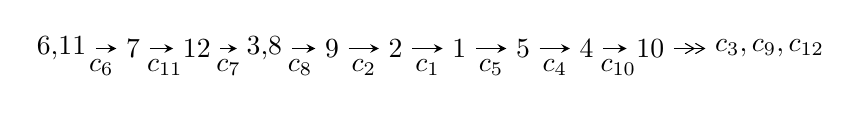
\begin{tikzpicture}[x=23pt, y=7pt]
	% node
	\node (A0) at (-1/8, 0) {6,11};
	\node (A1) at (1, 0) {7};
	\node (A2) at (2, 0) {12};
	\node (A3) at (49/16, 0) {3,8};
	\node (A4) at (33/8, 0) {9};
	\node (A5) at (41/8, 0) {2};
	\node (A6) at (49/8, 0) {1};
	\node (A7) at (57/8, 0) {5};
	\node (A8) at (65/8, 0) {4};
	\node (A9) at (73/8, 0) {10};
	\node (C1) at (1/2, -1) {$c_{6}$};
	\node (C2) at (3/2, -1) {$c_{11}$};
	\node (C3) at (5/2, -1) {$c_{7}$};
	\node (C4) at (29/8, -1) {$c_{8}$};
	\node (C5) at (37/8, -1) {$c_{2}$};
	\node (C6) at (45/8, -1) {$c_{1}$};
	\node (C7) at (53/8, -1) {$c_{5}$};
	\node (C8) at (61/8, -1) {$c_{4}$};
	\node (C9) at (69/8, -1) {$c_{10}$};
	\node (A10) at (11, 0) {$c_{3},c_{9},c_{12}$};

	% edge
	\draw[->,>=stealth]	
	(A0) edge (A1) (A1) edge (A2) (A2) edge (A3) (A3) edge (A4) (A4) edge (A5) (A5) edge (A6) (A6) edge (A7) (A7) edge (A8) (A8) edge (A9) ;
	\draw[->>,>={angle 60}]	
	(A9) edge (A10);
\end{tikzpicture} \\ 

\end{tabular} \\

\footnotetext{
The image of knot diagram is generated by the software ``\textbf{Draw programme}" developed by Andrew Bartholomew(\url{http://www.layer8.co.uk/maths/draw/index.htm\#Running-draw}), where we modified some parts for our purpose(\url{https://github.com/CATsTAILs/LinksPainter}).
}\phantom \\ \newline 
\centering \textbf{Ideals for irreducible components\footnotemark of $X_{\text{par}}$} 
 
\begin{align*}
I^u_{1}&=\langle 
-296878516 u^{31}-276724358 u^{30}+\cdots+441171721 b-537239537,\\
\phantom{I^u_{1}}&\phantom{= \langle  }-397220095 u^{31}-1740337107 u^{30}+\cdots+882343442 a-7870777298,\;u^{32}+2 u^{31}+\cdots+6 u+1\rangle \\
I^u_{2}&=\langle 
b-1,\;a^2+2 a-2 u-3,\;u^2+u-1\rangle \\
I^u_{3}&=\langle 
b+1,\;a-1,\;u^2- u-1\rangle \\
\\
\end{align*}
\raggedright * 3 irreducible components of $\dim_{\mathbb{C}}=0$, with total 38 representations.\\
\footnotetext{All coefficients of polynomials are rational numbers. But the coefficients are sometimes approximated in decimal forms when there is not enough margin.}
\newpage
\renewcommand{\arraystretch}{1}
\centering \section*{I. $I^u_{1}= \langle -2.97\times10^{8} u^{31}-2.77\times10^{8} u^{30}+\cdots+4.41\times10^{8} b-5.37\times10^{8},\;-3.97\times10^{8} u^{31}-1.74\times10^{9} u^{30}+\cdots+8.82\times10^{8} a-7.87\times10^{9},\;u^{32}+2 u^{31}+\cdots+6 u+1 \rangle$}
\flushleft \textbf{(i) Arc colorings}\\
\begin{tabular}{m{7pt} m{180pt} m{7pt} m{180pt} }
\flushright $a_{6}=$&$\begin{pmatrix}1\\0\end{pmatrix}$ \\
\flushright $a_{11}=$&$\begin{pmatrix}0\\u\end{pmatrix}$ \\
\flushright $a_{7}=$&$\begin{pmatrix}1\\- u^2\end{pmatrix}$ \\
\flushright $a_{12}=$&$\begin{pmatrix}u\\- u^3+u\end{pmatrix}$ \\
\flushright $a_{3}=$&$\begin{pmatrix}0.450188 u^{31}+1.97240 u^{30}+\cdots-8.67806 u+8.92031\\0.672932 u^{31}+0.627249 u^{30}+\cdots+0.391427 u+1.21776\end{pmatrix}$ \\
\flushright $a_{8}=$&$\begin{pmatrix}- u^2+1\\u^4-2 u^2\end{pmatrix}$ \\
\flushright $a_{9}=$&$\begin{pmatrix}-2.40634 u^{31}-3.60527 u^{30}+\cdots+10.8122 u-12.0712\\0.218460 u^{31}-0.291561 u^{30}+\cdots+2.47123 u-1.19894\end{pmatrix}$ \\
\flushright $a_{2}=$&$\begin{pmatrix}1.12312 u^{31}+2.59965 u^{30}+\cdots-8.28663 u+10.1381\\0.672932 u^{31}+0.627249 u^{30}+\cdots+0.391427 u+1.21776\end{pmatrix}$ \\
\flushright $a_{1}=$&$\begin{pmatrix}- u^5+2 u^3+u\\u^5-3 u^3+u\end{pmatrix}$ \\
\flushright $a_{5}=$&$\begin{pmatrix}-1.26155 u^{31}-2.69290 u^{30}+\cdots+10.8624 u-9.38644\\-1.03259 u^{31}-0.976097 u^{30}+\cdots-1.09592 u-1.51802\end{pmatrix}$ \\
\flushright $a_{4}=$&$\begin{pmatrix}-0.145728 u^{31}-1.66532 u^{30}+\cdots+12.4977 u-7.36530\\-1.43787 u^{31}-1.24356 u^{30}+\cdots-2.16974 u-1.82405\end{pmatrix}$ \\
\flushright $a_{10}=$&$\begin{pmatrix}- u\\u\end{pmatrix}$\\&\end{tabular}
\flushleft \textbf{(ii) Obstruction class $= -1$}\\~\\
\flushleft \textbf{(iii) Cusp Shapes $= -\frac{619975605}{441171721} u^{31}-\frac{1193144219}{441171721} u^{30}+\cdots+\frac{5092498689}{441171721} u+\frac{1186500205}{441171721}$}\\~\\
\newpage\renewcommand{\arraystretch}{1}
\flushleft \textbf{(iv) u-Polynomials at the component}\newline \\
\begin{tabular}{m{50pt}|m{274pt}}
Crossings & \hspace{64pt}u-Polynomials at each crossing \\
\hline $$\begin{aligned}c_{1}\end{aligned}$$&$\begin{aligned}
&u^{32}+37 u^{31}+\cdots+305 u+1
\end{aligned}$\\
\hline $$\begin{aligned}c_{2},c_{5}\end{aligned}$$&$\begin{aligned}
&u^{32}+3 u^{31}+\cdots-7 u-1
\end{aligned}$\\
\hline $$\begin{aligned}c_{3},c_{8},c_{9}\end{aligned}$$&$\begin{aligned}
&u^{32}+u^{31}+\cdots-4 u+4
\end{aligned}$\\
\hline $$\begin{aligned}c_{4}\end{aligned}$$&$\begin{aligned}
&u^{32}-3 u^{31}+\cdots+12 u-4
\end{aligned}$\\
\hline $$\begin{aligned}c_{6},c_{7},c_{10}\\c_{11}\end{aligned}$$&$\begin{aligned}
&u^{32}+2 u^{31}+\cdots+6 u+1
\end{aligned}$\\
\hline $$\begin{aligned}c_{12}\end{aligned}$$&$\begin{aligned}
&u^{32}+4 u^{31}+\cdots-20 u+1
\end{aligned}$\\
\hline
\end{tabular}\\~\\
\newpage\renewcommand{\arraystretch}{1}
\flushleft \textbf{(v) Riley Polynomials at the component}\newline \\
\begin{tabular}{m{50pt}|m{274pt}}
Crossings & \hspace{64pt}Riley Polynomials at each crossing \\
\hline $$\begin{aligned}c_{1}\end{aligned}$$&$\begin{aligned}
&y^{32}-77 y^{31}+\cdots-68569 y+1
\end{aligned}$\\
\hline $$\begin{aligned}c_{2},c_{5}\end{aligned}$$&$\begin{aligned}
&y^{32}-37 y^{31}+\cdots-305 y+1
\end{aligned}$\\
\hline $$\begin{aligned}c_{3},c_{8},c_{9}\end{aligned}$$&$\begin{aligned}
&y^{32}-27 y^{31}+\cdots-208 y+16
\end{aligned}$\\
\hline $$\begin{aligned}c_{4}\end{aligned}$$&$\begin{aligned}
&y^{32}+33 y^{31}+\cdots-336 y+16
\end{aligned}$\\
\hline $$\begin{aligned}c_{6},c_{7},c_{10}\\c_{11}\end{aligned}$$&$\begin{aligned}
&y^{32}-36 y^{31}+\cdots-56 y+1
\end{aligned}$\\
\hline $$\begin{aligned}c_{12}\end{aligned}$$&$\begin{aligned}
&y^{32}+36 y^{31}+\cdots-568 y+1
\end{aligned}$\\
\hline
\end{tabular}\\~\\
\newpage\flushleft \textbf{(vi) Complex Volumes and Cusp Shapes}
$$\begin{array}{c|c|c}  
\text{Solutions to }I^u_{1}& \I (\text{vol} + \sqrt{-1}CS) & \text{Cusp shape}\\
 \hline 
\begin{aligned}
u &= \phantom{-}0.647923 + 0.702860 I \\
a &= -0.11556 - 1.50516 I \\
b &= -1.60683 + 0.23584 I\end{aligned}
 & -5.40621 + 7.69916 I & \phantom{-}6.58632 - 5.74078 I \\ \hline\begin{aligned}
u &= \phantom{-}0.647923 - 0.702860 I \\
a &= -0.11556 + 1.50516 I \\
b &= -1.60683 - 0.23584 I\end{aligned}
 & -5.40621 - 7.69916 I & \phantom{-}6.58632 + 5.74078 I \\ \hline\begin{aligned}
u &= -0.934535\phantom{ +0.000000I} \\
a &= \phantom{-}0.920748\phantom{ +0.000000I} \\
b &= -1.27591\phantom{ +0.000000I}\end{aligned}
 & \phantom{-}0.214319\phantom{ +0.000000I} & \phantom{-}11.1130\phantom{ +0.000000I} \\ \hline\begin{aligned}
u &= -0.528252 + 0.752905 I \\
a &= \phantom{-}0.219575 - 1.040740 I \\
b &= \phantom{-}1.65258 + 0.07144 I\end{aligned}
 & -9.84928 - 2.50165 I & \phantom{-}2.86477 + 2.84418 I \\ \hline\begin{aligned}
u &= -0.528252 - 0.752905 I \\
a &= \phantom{-}0.219575 + 1.040740 I \\
b &= \phantom{-}1.65258 - 0.07144 I\end{aligned}
 & -9.84928 + 2.50165 I & \phantom{-}2.86477 - 2.84418 I \\ \hline\begin{aligned}
u &= \phantom{-}0.383863 + 0.766338 I \\
a &= -0.382365 - 0.514382 I \\
b &= -1.62188 - 0.11406 I\end{aligned}
 & -6.19158 - 2.80814 I & \phantom{-}5.10038 + 0.76938 I \\ \hline\begin{aligned}
u &= \phantom{-}0.383863 - 0.766338 I \\
a &= -0.382365 + 0.514382 I \\
b &= -1.62188 + 0.11406 I\end{aligned}
 & -6.19158 + 2.80814 I & \phantom{-}5.10038 - 0.76938 I \\ \hline\begin{aligned}
u &= -0.750792\phantom{ +0.000000I} \\
a &= -1.84633\phantom{ +0.000000I} \\
b &= \phantom{-}0.310110\phantom{ +0.000000I}\end{aligned}
 & \phantom{-}5.68749\phantom{ +0.000000I} & \phantom{-}17.7080\phantom{ +0.000000I} \\ \hline\begin{aligned}
u &= \phantom{-}0.505153 + 0.538065 I \\
a &= \phantom{-}0.446790 + 1.310620 I \\
b &= \phantom{-}0.571805 - 0.732824 I\end{aligned}
 & \phantom{-}1.93515 + 4.07265 I & \phantom{-}8.92952 - 7.04568 I \\ \hline\begin{aligned}
u &= \phantom{-}0.505153 - 0.538065 I \\
a &= \phantom{-}0.446790 - 1.310620 I \\
b &= \phantom{-}0.571805 + 0.732824 I\end{aligned}
 & \phantom{-}1.93515 - 4.07265 I & \phantom{-}8.92952 + 7.04568 I\\
 \hline 
 \end{array}$$\newpage$$\begin{array}{c|c|c}  
\text{Solutions to }I^u_{1}& \I (\text{vol} + \sqrt{-1}CS) & \text{Cusp shape}\\
 \hline 
\begin{aligned}
u &= \phantom{-}0.395138 + 0.481331 I \\
a &= -0.551243 - 0.194239 I \\
b &= \phantom{-}0.642691 + 0.571386 I\end{aligned}
 & \phantom{-}1.68006 - 0.53375 I & \phantom{-}7.96422 - 0.32995 I \\ \hline\begin{aligned}
u &= \phantom{-}0.395138 - 0.481331 I \\
a &= -0.551243 + 0.194239 I \\
b &= \phantom{-}0.642691 - 0.571386 I\end{aligned}
 & \phantom{-}1.68006 + 0.53375 I & \phantom{-}7.96422 + 0.32995 I \\ \hline\begin{aligned}
u &= -1.40514 + 0.25786 I \\
a &= \phantom{-}0.848313 + 0.771560 I \\
b &= -1.59035 - 0.06318 I\end{aligned}
 & -0.512682 - 0.890588 I & \phantom{-}8.15263 + 0. I\phantom{ +0.000000I} \\ \hline\begin{aligned}
u &= -1.40514 - 0.25786 I \\
a &= \phantom{-}0.848313 - 0.771560 I \\
b &= -1.59035 + 0.06318 I\end{aligned}
 & -0.512682 + 0.890588 I & \phantom{-}8.15263 + 0. I\phantom{ +0.000000I} \\ \hline\begin{aligned}
u &= \phantom{-}1.44428 + 0.09174 I \\
a &= \phantom{-}0.42149 - 1.57076 I \\
b &= -0.611773 + 0.763659 I\end{aligned}
 & \phantom{-}4.34598 + 2.60375 I & \phantom{-}7.93484 - 3.36675 I \\ \hline\begin{aligned}
u &= \phantom{-}1.44428 - 0.09174 I \\
a &= \phantom{-}0.42149 + 1.57076 I \\
b &= -0.611773 - 0.763659 I\end{aligned}
 & \phantom{-}4.34598 - 2.60375 I & \phantom{-}7.93484 + 3.36675 I \\ \hline\begin{aligned}
u &= \phantom{-}1.44949\phantom{ +0.000000I} \\
a &= \phantom{-}0.265813\phantom{ +0.000000I} \\
b &= \phantom{-}1.38846\phantom{ +0.000000I}\end{aligned}
 & \phantom{-}8.83218\phantom{ +0.000000I} & \phantom{-}9.93110\phantom{ +0.000000I} \\ \hline\begin{aligned}
u &= -1.45288 + 0.07180 I \\
a &= -0.88013 + 1.22133 I \\
b &= \phantom{-}0.795382 - 0.670343 I\end{aligned}
 & \phantom{-}7.57700 - 1.16778 I & \phantom{-}11.36341 + 0.54162 I \\ \hline\begin{aligned}
u &= -1.45288 - 0.07180 I \\
a &= -0.88013 - 1.22133 I \\
b &= \phantom{-}0.795382 + 0.670343 I\end{aligned}
 & \phantom{-}7.57700 + 1.16778 I & \phantom{-}11.36341 - 0.54162 I \\ \hline\begin{aligned}
u &= -1.51955 + 0.16796 I \\
a &= -0.08132 - 1.78171 I \\
b &= \phantom{-}0.464019 + 0.904411 I\end{aligned}
 & \phantom{-}8.62955 - 6.62987 I & \phantom{-}12.50269 + 5.26876 I\\
 \hline 
 \end{array}$$\newpage$$\begin{array}{c|c|c}  
\text{Solutions to }I^u_{1}& \I (\text{vol} + \sqrt{-1}CS) & \text{Cusp shape}\\
 \hline 
\begin{aligned}
u &= -1.51955 - 0.16796 I \\
a &= -0.08132 + 1.78171 I \\
b &= \phantom{-}0.464019 - 0.904411 I\end{aligned}
 & \phantom{-}8.62955 + 6.62987 I & \phantom{-}12.50269 - 5.26876 I \\ \hline\begin{aligned}
u &= -0.299017 + 0.362824 I \\
a &= -0.106458 + 1.400860 I \\
b &= -0.751935 - 0.325766 I\end{aligned}
 & -1.32881 - 1.04587 I & \phantom{-}0.13410 + 4.26985 I \\ \hline\begin{aligned}
u &= -0.299017 - 0.362824 I \\
a &= -0.106458 - 1.400860 I \\
b &= -0.751935 + 0.325766 I\end{aligned}
 & -1.32881 + 1.04587 I & \phantom{-}0.13410 - 4.26985 I \\ \hline\begin{aligned}
u &= \phantom{-}1.52451 + 0.26507 I \\
a &= -0.93070 + 1.22794 I \\
b &= \phantom{-}1.61492 - 0.22198 I\end{aligned}
 & -3.16368 + 6.23347 I & \phantom{-}6.00000 - 3.63332 I \\ \hline\begin{aligned}
u &= \phantom{-}1.52451 - 0.26507 I \\
a &= -0.93070 - 1.22794 I \\
b &= \phantom{-}1.61492 + 0.22198 I\end{aligned}
 & -3.16368 - 6.23347 I & \phantom{-}6.00000 + 3.63332 I \\ \hline\begin{aligned}
u &= \phantom{-}0.451835\phantom{ +0.000000I} \\
a &= \phantom{-}0.432993\phantom{ +0.000000I} \\
b &= \phantom{-}0.202201\phantom{ +0.000000I}\end{aligned}
 & \phantom{-}0.642131\phantom{ +0.000000I} & \phantom{-}15.9520\phantom{ +0.000000I} \\ \hline\begin{aligned}
u &= -1.58469\phantom{ +0.000000I} \\
a &= -0.466896\phantom{ +0.000000I} \\
b &= \phantom{-}0.692717\phantom{ +0.000000I}\end{aligned}
 & \phantom{-}7.78318\phantom{ +0.000000I} & \phantom{-}17.5750\phantom{ +0.000000I} \\ \hline\begin{aligned}
u &= -1.58841 + 0.23470 I \\
a &= \phantom{-}0.92703 + 1.56136 I \\
b &= -1.56211 - 0.33651 I\end{aligned}
 & \phantom{-}2.01653 - 11.20740 I & \phantom{-0.000000 } 0 \\ \hline\begin{aligned}
u &= -1.58841 - 0.23470 I \\
a &= \phantom{-}0.92703 - 1.56136 I \\
b &= -1.56211 + 0.33651 I\end{aligned}
 & \phantom{-}2.01653 + 11.20740 I & \phantom{-0.000000 } 0 \\ \hline\begin{aligned}
u &= \phantom{-}1.61270\phantom{ +0.000000I} \\
a &= -0.848466\phantom{ +0.000000I} \\
b &= -0.0619566\phantom{ +0.000000I}\end{aligned}
 & \phantom{-}13.8091\phantom{ +0.000000I} & \phantom{-}18.0020\phantom{ +0.000000I}\\
 \hline 
 \end{array}$$\newpage$$\begin{array}{c|c|c}  
\text{Solutions to }I^u_{1}& \I (\text{vol} + \sqrt{-1}CS) & \text{Cusp shape}\\
 \hline 
\begin{aligned}
u &= \phantom{-}1.68667\phantom{ +0.000000I} \\
a &= \phantom{-}1.46963\phantom{ +0.000000I} \\
b &= -1.31101\phantom{ +0.000000I}\end{aligned}
 & \phantom{-}9.57646\phantom{ +0.000000I} & \phantom{-}6.00000\phantom{ +0.000000I} \\ \hline\begin{aligned}
u &= -0.145893\phantom{ +0.000000I} \\
a &= \phantom{-}9.44166\phantom{ +0.000000I} \\
b &= \phantom{-}1.06237\phantom{ +0.000000I}\end{aligned}
 & \phantom{-}3.33910\phantom{ +0.000000I} & \phantom{-}1.65970\phantom{ +0.000000I}\\
 \hline 
 \end{array}$$\newpage\newpage\renewcommand{\arraystretch}{1}
\centering \section*{II. $I^u_{2}= \langle b-1,\;a^2+2 a-2 u-3,\;u^2+u-1 \rangle$}
\flushleft \textbf{(i) Arc colorings}\\
\begin{tabular}{m{7pt} m{180pt} m{7pt} m{180pt} }
\flushright $a_{6}=$&$\begin{pmatrix}1\\0\end{pmatrix}$ \\
\flushright $a_{11}=$&$\begin{pmatrix}0\\u\end{pmatrix}$ \\
\flushright $a_{7}=$&$\begin{pmatrix}1\\u-1\end{pmatrix}$ \\
\flushright $a_{12}=$&$\begin{pmatrix}u\\- u+1\end{pmatrix}$ \\
\flushright $a_{3}=$&$\begin{pmatrix}a\\1\end{pmatrix}$ \\
\flushright $a_{8}=$&$\begin{pmatrix}u\\- u\end{pmatrix}$ \\
\flushright $a_{9}=$&$\begin{pmatrix}a u-2\\- a u-2 u\end{pmatrix}$ \\
\flushright $a_{2}=$&$\begin{pmatrix}a+1\\1\end{pmatrix}$ \\
\flushright $a_{1}=$&$\begin{pmatrix}1\\0\end{pmatrix}$ \\
\flushright $a_{5}=$&$\begin{pmatrix}- a\\-1\end{pmatrix}$ \\
\flushright $a_{4}=$&$\begin{pmatrix}- a u- u+1\\a u- a+u-2\end{pmatrix}$ \\
\flushright $a_{10}=$&$\begin{pmatrix}- u\\u\end{pmatrix}$\\&\end{tabular}
\flushleft \textbf{(ii) Obstruction class $= 1$}\\~\\
\flushleft \textbf{(iii) Cusp Shapes $= 12$}\\~\\
\newpage\renewcommand{\arraystretch}{1}
\flushleft \textbf{(iv) u-Polynomials at the component}\newline \\
\begin{tabular}{m{50pt}|m{274pt}}
Crossings & \hspace{64pt}u-Polynomials at each crossing \\
\hline $$\begin{aligned}c_{1},c_{5}\end{aligned}$$&$\begin{aligned}
&(u-1)^4
\end{aligned}$\\
\hline $$\begin{aligned}c_{2}\end{aligned}$$&$\begin{aligned}
&(u+1)^4
\end{aligned}$\\
\hline $$\begin{aligned}c_{3},c_{4},c_{8}\\c_{9}\end{aligned}$$&$\begin{aligned}
&(u^2-2)^2
\end{aligned}$\\
\hline $$\begin{aligned}c_{6},c_{7},c_{12}\end{aligned}$$&$\begin{aligned}
&(u^2+u-1)^2
\end{aligned}$\\
\hline $$\begin{aligned}c_{10},c_{11}\end{aligned}$$&$\begin{aligned}
&(u^2- u-1)^2
\end{aligned}$\\
\hline
\end{tabular}\\~\\
\newpage\renewcommand{\arraystretch}{1}
\flushleft \textbf{(v) Riley Polynomials at the component}\newline \\
\begin{tabular}{m{50pt}|m{274pt}}
Crossings & \hspace{64pt}Riley Polynomials at each crossing \\
\hline $$\begin{aligned}c_{1},c_{2},c_{5}\end{aligned}$$&$\begin{aligned}
&(y-1)^4
\end{aligned}$\\
\hline $$\begin{aligned}c_{3},c_{4},c_{8}\\c_{9}\end{aligned}$$&$\begin{aligned}
&(y-2)^4
\end{aligned}$\\
\hline $$\begin{aligned}c_{6},c_{7},c_{10}\\c_{11},c_{12}\end{aligned}$$&$\begin{aligned}
&(y^2-3 y+1)^2
\end{aligned}$\\
\hline
\end{tabular}\\~\\
\newpage\flushleft \textbf{(vi) Complex Volumes and Cusp Shapes}
$$\begin{array}{c|c|c}  
\text{Solutions to }I^u_{2}& \I (\text{vol} + \sqrt{-1}CS) & \text{Cusp shape}\\
 \hline 
\begin{aligned}
u &= \phantom{-}0.618034\phantom{ +0.000000I} \\
a &= \phantom{-}1.28825\phantom{ +0.000000I} \\
b &= \phantom{-}1.00000\phantom{ +0.000000I}\end{aligned}
 & \phantom{-}4.27683\phantom{ +0.000000I} & \phantom{-}12.0000\phantom{ +0.000000I} \\ \hline\begin{aligned}
u &= \phantom{-}0.618034\phantom{ +0.000000I} \\
a &= -3.28825\phantom{ +0.000000I} \\
b &= \phantom{-}1.00000\phantom{ +0.000000I}\end{aligned}
 & \phantom{-}4.27683\phantom{ +0.000000I} & \phantom{-}12.0000\phantom{ +0.000000I} \\ \hline\begin{aligned}
u &= -1.61803\phantom{ +0.000000I} \\
a &= -0.125968\phantom{ +0.000000I} \\
b &= \phantom{-}1.00000\phantom{ +0.000000I}\end{aligned}
 & \phantom{-}12.1725\phantom{ +0.000000I} & \phantom{-}12.0000\phantom{ +0.000000I} \\ \hline\begin{aligned}
u &= -1.61803\phantom{ +0.000000I} \\
a &= -1.87403\phantom{ +0.000000I} \\
b &= \phantom{-}1.00000\phantom{ +0.000000I}\end{aligned}
 & \phantom{-}12.1725\phantom{ +0.000000I} & \phantom{-}12.0000\phantom{ +0.000000I}\\
 \hline 
 \end{array}$$\newpage\newpage\renewcommand{\arraystretch}{1}
\centering \section*{III. $I^u_{3}= \langle b+1,\;a-1,\;u^2- u-1 \rangle$}
\flushleft \textbf{(i) Arc colorings}\\
\begin{tabular}{m{7pt} m{180pt} m{7pt} m{180pt} }
\flushright $a_{6}=$&$\begin{pmatrix}1\\0\end{pmatrix}$ \\
\flushright $a_{11}=$&$\begin{pmatrix}0\\u\end{pmatrix}$ \\
\flushright $a_{7}=$&$\begin{pmatrix}1\\- u-1\end{pmatrix}$ \\
\flushright $a_{12}=$&$\begin{pmatrix}u\\- u-1\end{pmatrix}$ \\
\flushright $a_{3}=$&$\begin{pmatrix}1\\-1\end{pmatrix}$ \\
\flushright $a_{8}=$&$\begin{pmatrix}- u\\u\end{pmatrix}$ \\
\flushright $a_{9}=$&$\begin{pmatrix}- u\\u\end{pmatrix}$ \\
\flushright $a_{2}=$&$\begin{pmatrix}0\\-1\end{pmatrix}$ \\
\flushright $a_{1}=$&$\begin{pmatrix}-1\\0\end{pmatrix}$ \\
\flushright $a_{5}=$&$\begin{pmatrix}1\\-1\end{pmatrix}$ \\
\flushright $a_{4}=$&$\begin{pmatrix}1\\-1\end{pmatrix}$ \\
\flushright $a_{10}=$&$\begin{pmatrix}- u\\u\end{pmatrix}$\\&\end{tabular}
\flushleft \textbf{(ii) Obstruction class $= 1$}\\~\\
\flushleft \textbf{(iii) Cusp Shapes $= 2$}\\~\\
\newpage\renewcommand{\arraystretch}{1}
\flushleft \textbf{(iv) u-Polynomials at the component}\newline \\
\begin{tabular}{m{50pt}|m{274pt}}
Crossings & \hspace{64pt}u-Polynomials at each crossing \\
\hline $$\begin{aligned}c_{1},c_{2}\end{aligned}$$&$\begin{aligned}
&(u-1)^2
\end{aligned}$\\
\hline $$\begin{aligned}c_{3},c_{4},c_{8}\\c_{9}\end{aligned}$$&$\begin{aligned}
&u^2
\end{aligned}$\\
\hline $$\begin{aligned}c_{5}\end{aligned}$$&$\begin{aligned}
&(u+1)^2
\end{aligned}$\\
\hline $$\begin{aligned}c_{6},c_{7}\end{aligned}$$&$\begin{aligned}
&u^2- u-1
\end{aligned}$\\
\hline $$\begin{aligned}c_{10},c_{11},c_{12}\end{aligned}$$&$\begin{aligned}
&u^2+u-1
\end{aligned}$\\
\hline
\end{tabular}\\~\\
\newpage\renewcommand{\arraystretch}{1}
\flushleft \textbf{(v) Riley Polynomials at the component}\newline \\
\begin{tabular}{m{50pt}|m{274pt}}
Crossings & \hspace{64pt}Riley Polynomials at each crossing \\
\hline $$\begin{aligned}c_{1},c_{2},c_{5}\end{aligned}$$&$\begin{aligned}
&(y-1)^2
\end{aligned}$\\
\hline $$\begin{aligned}c_{3},c_{4},c_{8}\\c_{9}\end{aligned}$$&$\begin{aligned}
&y^2
\end{aligned}$\\
\hline $$\begin{aligned}c_{6},c_{7},c_{10}\\c_{11},c_{12}\end{aligned}$$&$\begin{aligned}
&y^2-3 y+1
\end{aligned}$\\
\hline
\end{tabular}\\~\\
\newpage\flushleft \textbf{(vi) Complex Volumes and Cusp Shapes}
$$\begin{array}{c|c|c}  
\text{Solutions to }I^u_{3}& \I (\text{vol} + \sqrt{-1}CS) & \text{Cusp shape}\\
 \hline 
\begin{aligned}
u &= -0.618034\phantom{ +0.000000I} \\
a &= \phantom{-}1.00000\phantom{ +0.000000I} \\
b &= -1.00000\phantom{ +0.000000I}\end{aligned}
 & -0.657974\phantom{ +0.000000I} & \phantom{-}2.00000\phantom{ +0.000000I} \\ \hline\begin{aligned}
u &= \phantom{-}1.61803\phantom{ +0.000000I} \\
a &= \phantom{-}1.00000\phantom{ +0.000000I} \\
b &= -1.00000\phantom{ +0.000000I}\end{aligned}
 & \phantom{-}7.23771\phantom{ +0.000000I} & \phantom{-}2.00000\phantom{ +0.000000I}\\
 \hline 
 \end{array}$$\newpage
\newpage\renewcommand{\arraystretch}{1}
\centering \section*{ IV. u-Polynomials}
\begin{tabular}{m{50pt}|m{274pt}}
Crossings & \hspace{64pt}u-Polynomials at each crossing \\
\hline $$\begin{aligned}c_{1}\end{aligned}$$&$\begin{aligned}
&((u-1)^6)(u^{32}+37 u^{31}+\cdots+305 u+1)
\end{aligned}$\\
\hline $$\begin{aligned}c_{2}\end{aligned}$$&$\begin{aligned}
&((u-1)^2)(u+1)^4(u^{32}+3 u^{31}+\cdots-7 u-1)
\end{aligned}$\\
\hline $$\begin{aligned}c_{3},c_{8},c_{9}\end{aligned}$$&$\begin{aligned}
&u^2(u^2-2)^2(u^{32}+u^{31}+\cdots-4 u+4)
\end{aligned}$\\
\hline $$\begin{aligned}c_{4}\end{aligned}$$&$\begin{aligned}
&u^2(u^2-2)^2(u^{32}-3 u^{31}+\cdots+12 u-4)
\end{aligned}$\\
\hline $$\begin{aligned}c_{5}\end{aligned}$$&$\begin{aligned}
&((u-1)^4)(u+1)^2(u^{32}+3 u^{31}+\cdots-7 u-1)
\end{aligned}$\\
\hline $$\begin{aligned}c_{6},c_{7}\end{aligned}$$&$\begin{aligned}
&(u^2- u-1)(u^2+u-1)^2(u^{32}+2 u^{31}+\cdots+6 u+1)
\end{aligned}$\\
\hline $$\begin{aligned}c_{10},c_{11}\end{aligned}$$&$\begin{aligned}
&((u^2- u-1)^2)(u^2+u-1)(u^{32}+2 u^{31}+\cdots+6 u+1)
\end{aligned}$\\
\hline $$\begin{aligned}c_{12}\end{aligned}$$&$\begin{aligned}
&((u^2+u-1)^3)(u^{32}+4 u^{31}+\cdots-20 u+1)
\end{aligned}$\\
\hline
\end{tabular}\newpage\renewcommand{\arraystretch}{1}
\centering \section*{ V. Riley Polynomials}
\begin{tabular}{m{50pt}|m{274pt}}
Crossings & \hspace{64pt}Riley Polynomials at each crossing \\
\hline $$\begin{aligned}c_{1}\end{aligned}$$&$\begin{aligned}
&((y-1)^6)(y^{32}-77 y^{31}+\cdots-68569 y+1)
\end{aligned}$\\
\hline $$\begin{aligned}c_{2},c_{5}\end{aligned}$$&$\begin{aligned}
&((y-1)^6)(y^{32}-37 y^{31}+\cdots-305 y+1)
\end{aligned}$\\
\hline $$\begin{aligned}c_{3},c_{8},c_{9}\end{aligned}$$&$\begin{aligned}
&y^2(y-2)^4(y^{32}-27 y^{31}+\cdots-208 y+16)
\end{aligned}$\\
\hline $$\begin{aligned}c_{4}\end{aligned}$$&$\begin{aligned}
&y^2(y-2)^4(y^{32}+33 y^{31}+\cdots-336 y+16)
\end{aligned}$\\
\hline $$\begin{aligned}c_{6},c_{7},c_{10}\\c_{11}\end{aligned}$$&$\begin{aligned}
&((y^2-3 y+1)^3)(y^{32}-36 y^{31}+\cdots-56 y+1)
\end{aligned}$\\
\hline $$\begin{aligned}c_{12}\end{aligned}$$&$\begin{aligned}
&((y^2-3 y+1)^3)(y^{32}+36 y^{31}+\cdots-568 y+1)
\end{aligned}$\\
\hline
\end{tabular}
\vskip 2pc
\end{document}